\chapter{Estudo de Caso}

Neste capítulo será apresentado o estudo de caso sobre a utilização de práticas de usabilidade e testes automatizados no desenvolvimento do Portal do Software Público, baseado na plataforma Noosfero, onde será definido um guia de como essas práticas podem ser inseridas nesse contexto específico.

\section{Objeto de Estudo: Portal do Software Público Brasileiro - SPB}

O Portal do Software Público Brasileiro consiste em um sistema que permite o compartilhamento de softwares e faz parte da política de software livre no setor público.
O SPB será o objeto de estudo de caso, assim como o processo de colaboração com o SPB, que é realizado no LAPPIS da UnB.

\subsection{Visão Geral do Projeto}

O processo de colaboração com o SPB baseia-se no desenvolvimento empírico e nas metodologias ágeis scrum e XP. O desenvolvimento de testes automatizados é intrínseco ao processo de desenvolvimento. A partir destes pontos mencionados, buscamos evoluir a forma com que o processo de colaboraçao com o SPB lida com problemas de usabilidade.
O processo de desenvolvimento é feito a partir de sprints de duas semanas, em que são realizadas reuniões com as equipes e reuniões de planejamento (Planning Poker) em cada equipe para definir as atividades de cada sprint.

%Explicar a dinâmica de trabalho, a equipe, reuniões
%verificar aonde vai entrar essa seção. Talvex dentro do contexto?


 
\section{Execução}

\subsection{Práticas adotadas}


No acompanhamento do projeto podemos identificar inicialmente os seguintes problemas relacionados à usabilidade no desenvolvimento de software:

\textbf{Questionário Online}

Inicialmente à equipe de design realizou um planejamento para definir o instrumento de pesquisa dos usuários. Foi definido que o principal objetivo do estudo seria medir a percepção dos usuários quanto a qualidade de uso do portal atual sob uma perspectiva global. Nesse sentido foi proposto uma abordagem de pesquisa de levantamento aplicada e quantitativa. A qualidade de uso foi compreendida a partir dos parâmetros propostos pela ISO 9241-10 a 17, como a qualidade da interface de proporcionar eficácia, eficiência e satisfação no uso do portal (APPOLINÁRIO, 2004). 

Na definição do delineamento da pesquisa foi selecionada a técnica de aplicação de questionário on-line para se produzir os dados de opinião dos participantes. Entende-se que a dimensão atitudinal dos usuários do portal com relação a sua experiência de uso só podem ser obtidos por meio do registro de suas verbalizações (MARTINS E THEOPHILO, 2009). No mesmo sentido, a avaliação proposta não permite uma compreensão direta e completa a cerca da usabilidade do portal em si, compreendendo-se que a efetividade do portal só pode ser analisada 
diretamente por meio do uso de outras técnicas de pesquisa, como as observações globais ou sistemáticas da interação entre os participantes e a sua interface % (MARTINS e THEÓPHILO, 2009; ABRAHÃO et al., 2009).


\textbf{Checklists}
	Foi desenvolvido um checklist para auxiliar nas avaliações de heurísticas (cada pergunta pode ser respondida em ``Sim'', ``Não'' e ``Não se aplica'', seguindo as seguintes características:
	\begin{itemize}
		\item \textbf{Prestreza:} uma boa presteza guia o usuário e lhe poupa, por exemplo, o aprendizado de uma série de comandos, permite, também, que o usuário saiba em que estado ele está, onde ele se encontra no diálogo e o que ele fez para se encontrar nessa situação. 
		
		\textbf{Questao 01:} Os títulos de telas, janelas e caixas de diálogo estão no alto, centrados ou justificados à esquerda? 
    
    	\textbf{Questão 02:} Caso o dado a entrar possua um formato particular, esse formato encontra-se descrito na tela?
    
    	\textbf{Questão 03:} Os rótulos dos campos contêm um elemento específico, por exemplo ``:'', como convite às entradas de dados?
    
    	\textbf{Questão 04:} O usuário encontra disponíveis as informações necessárias para suas ações?  

    	\item \textbf{Agrupamento por localização:} A compreensão de uma tela pelo usuário depende, entre outras coisas, da ordenação dos objetos que são apresentados. Os usuários irão detectar os diferentes itens mais facilmente se eles forem apresentados de uma forma organizada.

    	\textbf{Questão 01:} A disposição dos objetos de interação de uma caixa de dialogo segue uma ordem lógica?
	
    	\item \textbf{Agrupamento por formato:} Será mais fácil para o usuário perceber relacionamento(s) entre itens ou classes de itens, se diferentes formatos ou diferentes códigos ilustrarem suas similaridades ou diferenças.

	
    	\textbf{Questão 01:} Os diferentes tipos de elementos de uma tela de consulta (dados, comandos e instruções) são visualmente distintos uns dos outros?
   
   		\textbf{Questão 02:} Os cabeçalhos de uma tabela estão diferenciados através do emprego de cores diferentes, letras maiores ou sublinhadas?
	   
	   	\textbf{Questão 03:} Na apresentação de textos, os recursos de estilo, como itálico, negrito, sublinhado ou diferentes fontes são empregados para salientar palavras ou noções importantes
    
    	\textbf{Questão 04:} Os campos obrigatórios são diferenciados dos campos opcionais de forma visualmente clara? 
	    
	    \textbf{Questão 05:}  Nas caixas de mensagens, o botão selecionado por default tem uma apresentação visual suficientemente distinta dos outros? 

	    \item \textbf{Feedback:} A qualidade e a rapidez do feedback são dois fatores importantes para o estabelecimento de satisfação e confiança do usuário, assim como para o entendimento do diálogo.

    	\textbf{Questão 01:} O sistema fornece feedback para todas as ações do usuário? 
    
    	\textbf{Questão 02:} Quando, durante a entrada de dados, o sistema torna-se indisponível ao usuário, devido a algum processamento longo, o usuário é avisado desse estado do sistema e do tempo dessa indisponibilidade?
    
    	\textbf{Questão 03:} Os itens selecionados de uma lista são realçados visualmente de imediato? 
    
    	\item \textbf{Legibilidade:} A performance melhora quando a apresentação da informação leva em conta as características cognitivas e perceptivas dos usuários. Uma boa legibilidade facilita a leitura da informação apresentada. 

		\textbf{Questão 01:} As áreas livres são usadas para separar grupos lógicos em vez de tê-los todos de um só lado da tela, caixa ou janela?
     	
     	\textbf{Questão 02:} Os rótulos de campos organizados verticalmente e muito diferentes em tamanho estão justificados à direita?
     	
     	\textbf{Questão 03:} Os ícones são legíveis? 
     	
     	\item \textbf{Concisão:} Quanto menos entradas, menor a probabilidade de cometer erros. 

		\textbf{Questão 01:} O sistema oferece valores defaults para acelerar a entrada de dados?

		\item \textbf{Ações Mínimas:} Quanto mais numerosas e complexas forem as ações necessárias para se chegar a uma meta, a carga de trabalho aumentará e  a probabilidade de ocorrência de erros.

		\textbf{Questão 01:} Os grupos de botões de comando possuem sempre um botão definido como default? 

		\item \textbf{Controle do usuário:}	O controle sobre as interações favorece a aprendizagem e, assim, diminui a probabilidade de erros. 

		\textbf{Questão 01:} O usuário pode terminar um diálogo seqüencial repetitivo a qualquer instante? 
    
    	\textbf{Questão 02:} O usuário pode interromper e retomar um diálogo seqüencial a qualquer instante? 
	
    	\item \textbf{Proteção contra erros:} É preferível detectar os erros no momento da digitação, do que no momento da validação. Isto pode evitar perturbações na planificação da tarefa.

		\textbf{Questão 01:} O sistema apresenta uma separação adequada entre áreas selecionáveis de um painel de menu de modo a minimizar as ativações acidentais? 
    
    	\textbf{Questão 02:} Em toda ação destrutiva, os botões selecionados por default realizam a anulação dessa ação? 
   
   		\textbf{Questão 03:} O sistema solicita confirmação (dupla) de ações que podem gerar perdas de dados e/ou resultados catastróficos? 

   		\item \textbf{Mensagens de erro:} A qualidade das mensagens favorece o aprendizado do sistema, indicando ao usuário a razão ou a natureza do erro cometido, o que ele fez de errado, o que ele deveria ter feito e o que ele deve fazer.

		\textbf{Questão 01:} As mensagens de erro ajudam a resolver o problema do usuário, fornecendo com precisão o local e a causa específica ou provável do erro, bem como as ações que o usuário poderia realizar para corrigí-lo? 
    	
    	\textbf{Questão 02:} As frases das mensagens de erro são curtas e construídas a partir de palavras curtas, significativas e de uso comum? 

    	\item \textbf{Correção de erros:} Os erros são bem menos perturbadores quando eles são fáceis de corrigir.

		\textbf{Questão 01:} Qualquer ação do usuário pode ser revertida através da opção DESFAZER? 

		\item \textbf{Consistência:} Os procedimentos e rótulos são melhor reconhecidos quando seu formato são estáveis de uma tela para outra. Nessas condições, o sistema é mais previsível e a aprendizagem mais generalizável.

		\textbf{Questão 01:} A organização em termos da localização das várias características das janelas é mantida consistente de uma tela para outra? 
   
   		\textbf{Questão 02:} A localização dos dados é mantida consistente de uma tela para outra?  
   
   		\textbf{Questão 03:} Os formatos de apresentação dos dados são mantidos consistentes de uma tela para outra?

   		\textbf{Questão 04:} Os rótulos estão na mesma posição em relação aos campos associados?
	\end{itemize}

\textbf{Protótipos}
	A equipe utiliza-se de protótipos para determinar os cenários de uso do software, baseando-se nos requisitos definidos pelos clientes. Abaixo estão os protótipos de cadastro de usuário e cadastro de software:

	\begin{figure}[h!]
    	\centering
    	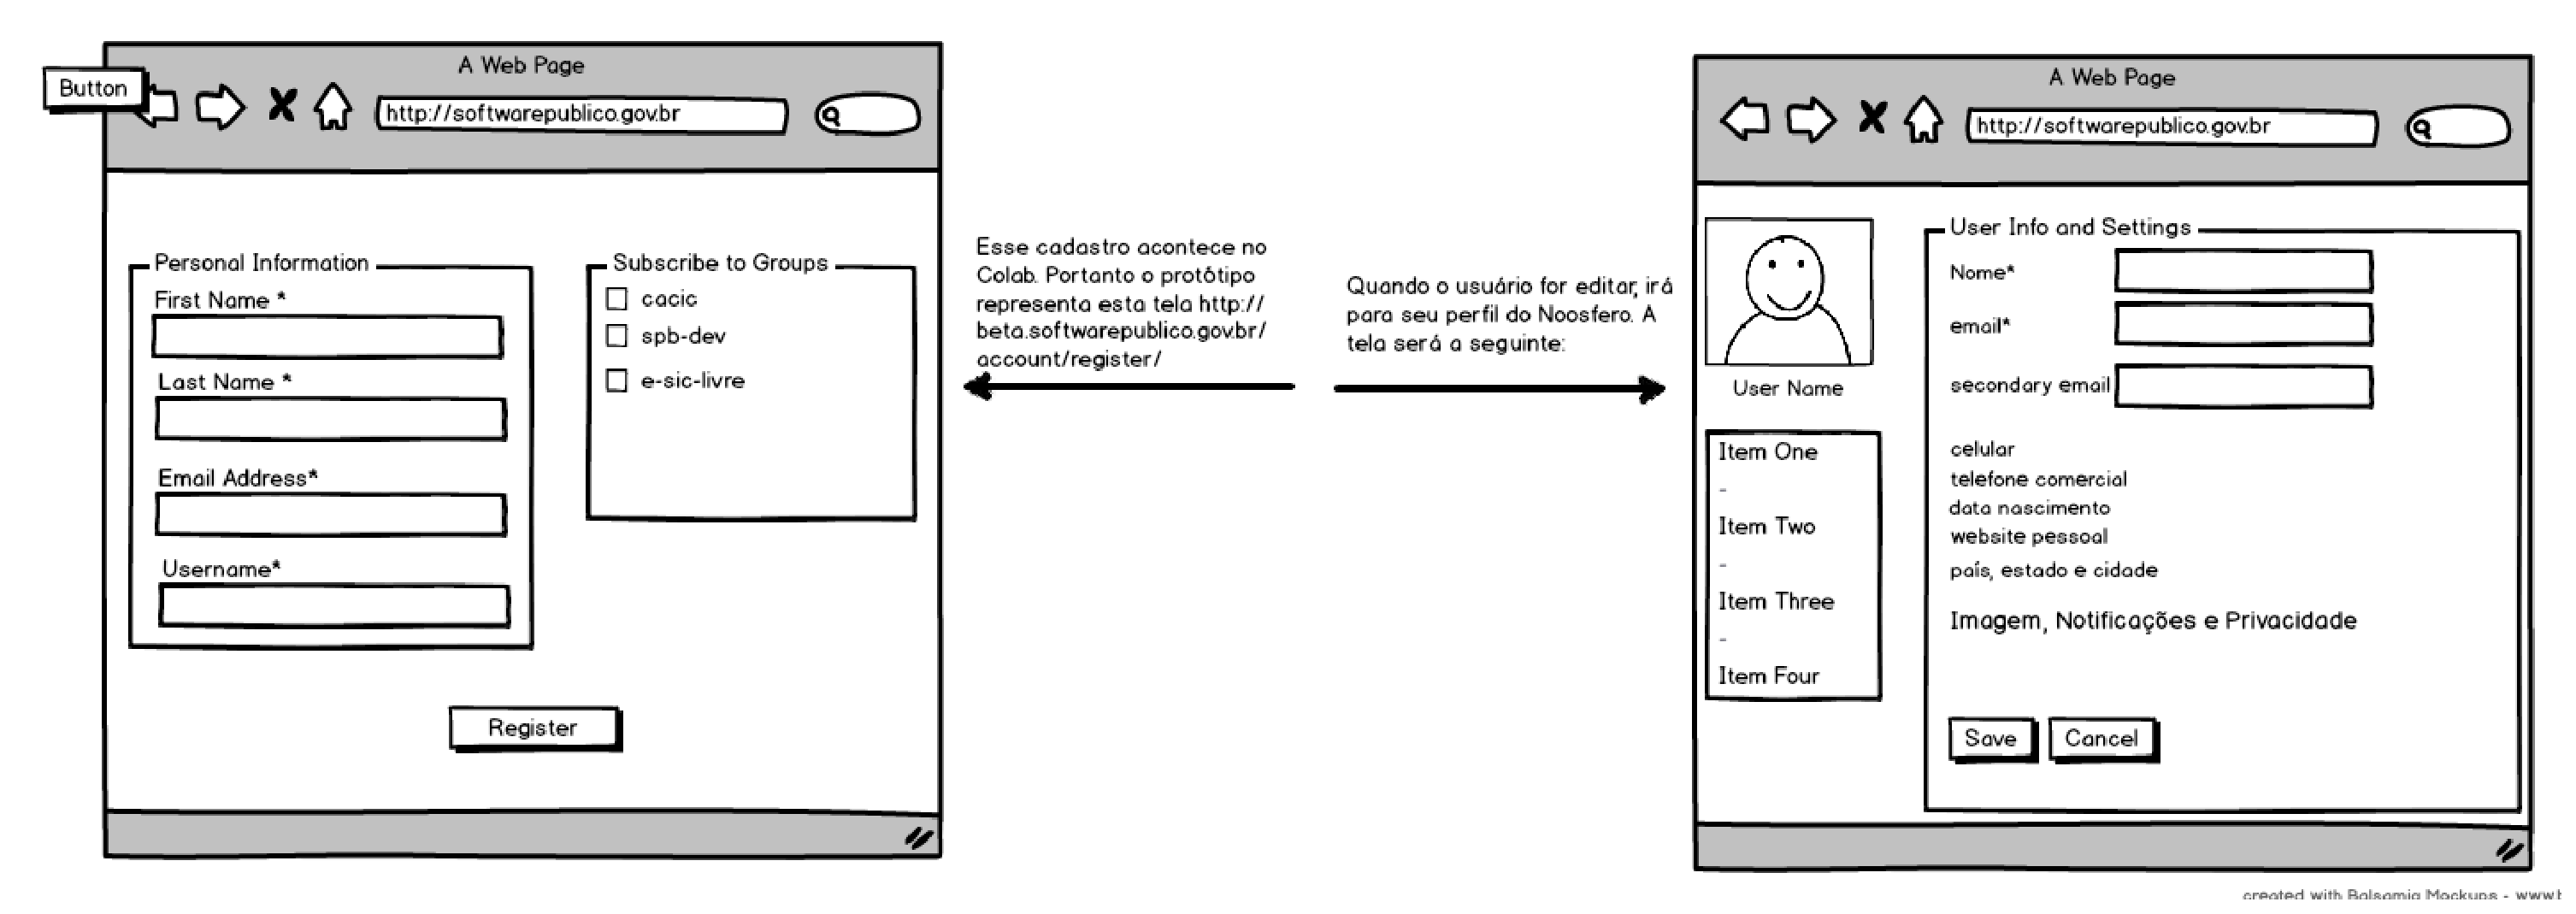
\includegraphics[keepaspectratio=true,scale=0.32]
      		{figuras/CadastroEdicaoUser.eps}
    	\caption{Protótipos de cadastro de usuário}
    	\label{cadastro user}
	\end{figure}

	\begin{figure}[h!]
    	\centering
    	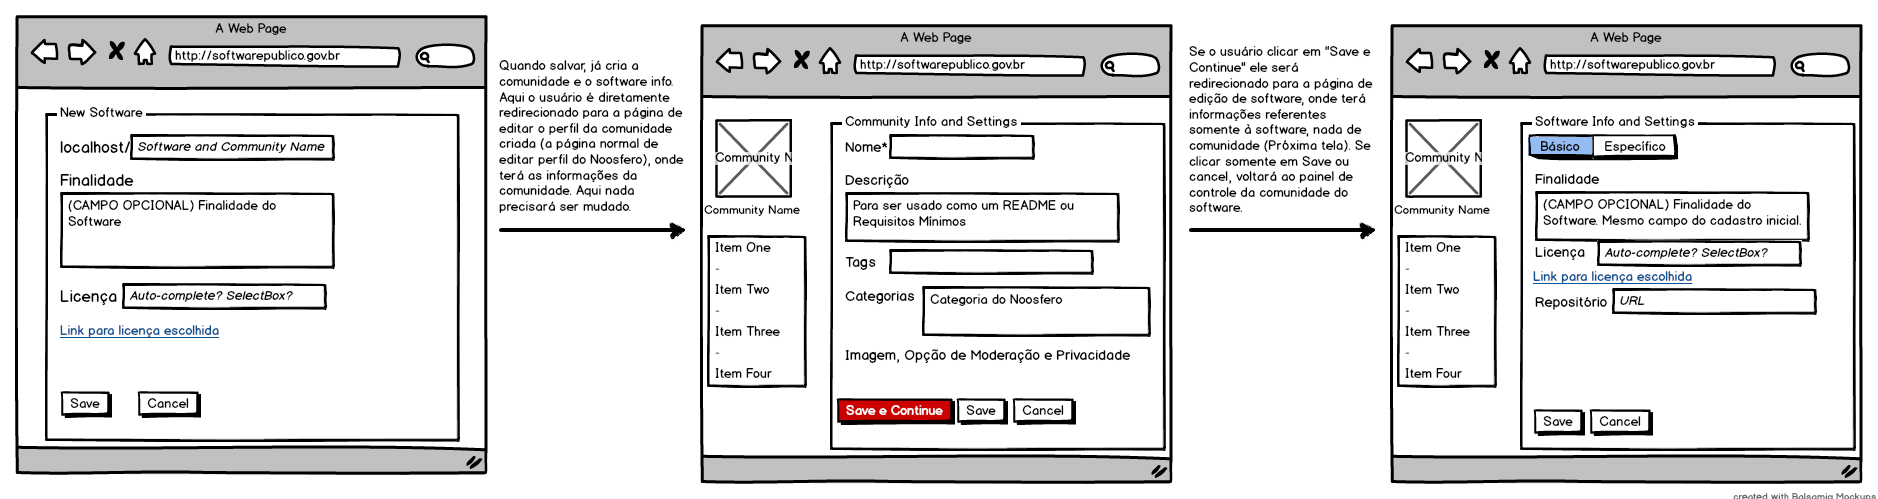
\includegraphics[keepaspectratio=true,scale=0.25]
      		{figuras/CadastroEdicaoSoftware.eps}
    	\caption{Protótipos de cadastro de software}
    	\label{cadastro software}
	\end{figure}

\newpage

\textbf{Cenários de Uso}
	Para cada funcionalidade desenvolvida é determinado um cenário de uso, base para a implementação dos testes de aceitação e consequentemente o desenvolvimento da funcionalidade propriamente dita.
	Durante a primeira release (release 0) foram desenvolvidas algumas histórias, dentre estas, a história de ``Cadastro de Usuário'', que possui os seguintes cenários de sucesso:

	\begin{itemize}
	\item\textbf{Cenário 01:} Cadastro com sucesso de apenas campos obrigatórios

	\textbf{[Dado]} que não existe nenhum usuário com o nome de usuário ``josesilva''

	\textbf{[Quando]} eu clicar em cadastrar novo usuário

	\textbf{[E]} eu preencho os seguintes campos: 

  		\subitem nome de usuário: ``josesilva''

  		\subitem e-mail: ``jose@gmail.com''

  		\subitem senha: ``123456''

  		\subitem confirmação da senha: ``123456''

  		\subitem nome completo: ``José da Silva''

  		\subitem país: ``Brasil''

  		\subitem estado: ``Distrito Federal''

  		\subitem cidade: ``Brasília''

	\textbf{[E]} eu clico em cadastrar

	\textbf{[Então]} eu recebo uma confirmação de cadastro realizado com sucesso


	\item\textbf{Cenário 02:} Cadastro com sucesso de apenas campos obrigatórios de usuário governamental
	
	\textbf{[Dado]} que não existe nenhum usuário com o nome de usuário ``josesilva''
	
	\textbf{[Quando]} eu clicar em cadastrar novo usuário
	
	\textbf{[E]} eu preencho os seguintes campos: 
  		\subitem nome de usuário: ``josesilva''

  		\subitem e-mail: ``jose@serpro.gov.br''

  		\subitem e-mail secundário: ``jose@gmail.com''

  		\subitem senha: ``123456''

		\subitem confirmação da senha: ``123456''

		\subitem nome completo: ``José da Silva''

		\subitem cargo: ``analista de TI''

		\subitem país: ``Brasil''

		 \subitem estado: ``Distrito Federal''

		\subitem cidade: ``Brasília''

	\textbf{[E]} eu seleciono ``SERPRO'' como instituição

	\textbf{[E]} eu seleciono ``????'' como unidade  

	\textbf{[E]} eu clico em cadastrar

	\textbf{[Então]}eu recebo uma confirmação de cadastro realizado com sucesso

\item\textbf{Cenário 3:} Cadastro com sucesso com todos os campos preenchidos, mesmo não obrigatórios

	\textbf{[Dado]} que não existe um usuário cujo email primário ou email secundário é ``maria@gmail.com''

	\textbf{[Quando]} eu clicar em cadastrar novo usuário

	\textbf{[E]} eu preencho os seguintes campos: 

  		\subitem nome de usuário: ``mariasilva''

		  \subitem e-mail: ``maria@gmail.com''

		  \subitem e-mail secundário: ``maria@yahoo.com''

		  \subitem senha: ``123456''

		  \subitem confirmação da senha: ``123456''

		  \subitem nome completo: ``Maria da Silva''

		  \subitem cargo: ``analista de TI''

		  \subitem áreas de interesse: ``Engenharia de Software''

		  \subitem país: ``Brasil''

		  \subitem estado: ``Distrito Federal''

		  \subitem cidade: ``Brasília''

	\textbf{[E]} eu seleciono ``Outro'' como instituição 

	\textbf{[E]} eu clico em cadastrar

	\textbf{[Então]} eu recebo uma notificação de cadastro realizado com sucesso.
	\end{itemize}

	Os cenários de falha ocorrem nas seguintes situações:
	\begin{itemize}
	\item Email proposto exisitir como email de outro usuário;
	\item Email secundário propostro exisitir como email de outro usuário;
	\item Email secundário ser um email governamental e ao email primário não ser um email governamental;
	\item Não preenchimento de campos obrigatórios para usuário governamental 
	\end{itemize}
%Especificar as datas, as atividades realizadas.


Outra funcionalidade desenvolvida foi a história chamada ``Manter Instituição'', que possui os seguintes cenários:
\begin{itemize}
\item\textbf{Cenário 01:} Cadastro de nova instituição com sucesso

\textbf{[Dado]} que eu estou na página de cadastro de usuário

\textbf{[E]} que a seguinte instituição não existe:

  	\subitem nome: ``Ministério do Planejamento, Orçamento e Gestão''

  	\subitem sigla: ``MP''

 	\subitem poder: ``executivo''

 	\subitem esfera: ``federal''

  	\subitem tipo: ``pública''

  	\subitem cnpj: ``00.489.828/0002-36''

\textbf{[Quando]} eu clicar em ``Cadastrar nova instituição''

\textbf{[E]} eu preencher os seguintes campos:

  	\subitem sigla: ``MP''

  	\subitem poder: ``executivo''

  	\subitem esfera: ``federal''

  	\subitem tipo: ``pública''

  	\subitem cnpj: ``00.489.828/0002-36''

\textbf{[Então]} eu devo visualizar a mensagem ``Instituição cadastrada com sucesso!''

\item\textbf{Cenário 02:} Busca de instituição inexistente

\textbf{[Dado]} que eu estou na página de cadastro de usuário

\textbf{[E]} que a seguinte instituição não existe:

 \subitem nome: ``Ministério do Planejamento, Orçamento e Gestão''

  \subitem sigla: ``MP''

  \subitem poder: ``executivo''

  \subitem esfera: ``federal''

  \subitem tipo: ``pública''
  
  \subitem cnpj: ``00.489.828/0002-36''

\textbf{[Quando]} eu buscar MP

\textbf{[Então]} eu devo visualizar a mensagem ``Instituição não cadastrada''

\textbf{[E]}eu devo visualizar a opção de cadastrar nova instituição
\end{itemize}

Estes cenários apresentam alguns problemas de usabilidade analisando-os de acordo com as heurísticas de Nielsen, e após o processo de desenvolvimento ter uma melhoria na visão de usabilidade após a incorporação de profissionais da área, os cenários apresentaram melhoras em relação às heurísticas de Nielsen. 

Durante a segunda release (release 1) as histórias de ``Cadastro de Usuário'', e ``Manter Instituição'' foram desenvolvidas novamente com os seguintes cenários:

\begin{itemize}
\item\textbf{Cenário 01:} Cadastro com sucesso de apenas campos obrigatórios

	\textbf{[Dado]} que não existe nenhum usuário com o nome de usuário ``josesilva''

	\textbf{[Quando]} eu clicar em ``Cadastre-se''

	\textbf{[E]} eu preencho os seguintes campos: 

  		\subitem primeiro nome: ``José''

  		\subitem ultimo nome: ``Silva''

  		\subitem endereço de e-mail: ``jose@gmail.com''

  		\subitem usuário: ``josesilva''
  		
	\textbf{[E]} eu clico em ``Cadastre-se''

	\textbf{[Então]} eu recebo uma confirmação de cadastro realizado com sucesso, com a seguinte mensgamte: 
	``Você deve se logar para seu perfil. Perfis não validados serão deletados em 24h.''
\end{itemize}

Para dar continuidade a este processo este estudo de caso avaliou os cenários estabelecidos e suas evoluções, verificando e propondo melhorias.

Durante a segunda release (release 2) a história de ``Novo Software'' foi desenvolvida com os seguintes cenários:

\begin{itemize}
\item\textbf{Cenário 01:} Novo Software

	\textbf{[Dado]} que não existe nenhum software com o localhost ``software''

	\textbf{[Quando]} eu clicar em ``Novo Software''

	\textbf{[E]} eu preencho os seguintes campos: 

  		\subitem localhost: ``software''

  		\subitem finalidade: ``Finalidade do software''

  		\subitem licenca: ``licença''
  		
  		
	\textbf{[E]} eu clico em ``Salvar''

	\textbf{[Então]} eu recebo uma confirmação de cadastro realizado com sucesso, e encontro a pagina de edição de software


Outros cenários de edição de software são: ``Informações de Comunidade'' e ``Informações de Software''.

\item\textbf{Cenário 02:} Informações de Comunidade

	\textbf{[Dado]} que ``software'' está cadastrado

	\textbf{[Quando]} eu clicar em ``Cadastre-se''

	\textbf{[E]} eu preencho os seguintes campos: 

  		\subitem descricao: ``Descricao do software''

  		\subitem tags: ``software''

  		\subitem categorias: ``categoria1''
 
	\textbf{[E]} eu clico em ``Salvar''

	\textbf{[Então]} eu recebo uma confirmação de cadastro salvo com sucesso


\item\textbf{Cenário 03:} Informações de Software

	\textbf{[Dado]} que ``software'' está cadastrado e estou em Edição de software

	\textbf{[Quando]} eu clicar em ``Especifico''

	\textbf{[E]} eu preencho os seguintes campos: 

  		\subitem Sigla: ``teste''

  		\subitem sistema operacional: ``teste os''

  		\subitem funcioanalidades: ``testes''

  		\subitem categorias: ``categoria1''
 	
 	\textbf{[E]} eu clico em ``Nova Biblioteca''

 	\textbf{[E]} eu preencho os seguintes campos: 

 		\subitem nome: ``teste''

 		\subitem versao: ``teste''

 		\subitem icenca: ``teste''

 	\textbf{[E]} eu clico em ``Novo Sistema Operacional''

 	\textbf{[E]} eu preencho os seguintes campos: 

 		\subitem nome: ``Debian''

 		\subitem versão: ``teste''

 	\textbf{[E]} eu clico em ``Nova linguagem''

 	\textbf{[E]} eu preencho os seguintes campos: 

 		\subitem nome: ``C++''

 		\subitem versão: ``teste''

 		\subitem sistema operacional: ``Debian''

 	\textbf{[E]} eu clico em ``Novo Banco de Dados''

 	\textbf{[E]} eu preencho os seguintes campos: 

 		\subitem nome: ``apache''

 		\subitem versão: ``teste''

 		\subitem sistema operacional: ``Debian''

	\textbf{[E]} eu clico em ``Salvar''

	\textbf{[Então]} eu recebo uma confirmação de cadastro salvo com sucesso

\end{itemize}


\textbf{Testes de Aceitação}

Os testes de aceitação software público são responsáveis por verificar os seguintes fatores:

\begin{itemize}
	\item Capacidade de registrar e editar informações de usuário e instituição;
	\item Capacidade de registrar e editar informações de software;
	\item Capacidade de desativar usuário;
	\item Capacidade de desativar software;
\end{itemize}


Segue abaixo os testes de aceitação desenvolvidos para e edição de software:

\textbf{Feature:} software registration
  As a user
  I want to create a new software
  So that I can have software communities on my network

  \textbf{Background:}

    \textbf{Given} ``MpogSoftwarePlugin'' plugin is enabled
  
    \textbf{And} SoftwareInfo has initial default values on database
  
    \textbf{And} I am logged in as admin
  
    \textbf{And} I go to /admin/plugins
  
    \textbf{And} I check ``MpogSoftwarePlugin''
  
    \textbf{And} I press ``Save changes''

  \textbf{Scenario:} Show library fields when click in New Library
  
    \textbf{Given} I go to admin user's control panel
  
    \textbf{And} I follow ``Manage my groups''
  
    \textbf{And} I follow ``Create a new software''
  
    \textbf{And} I follow ``New Library''
  
    \textbf{Then} I should see ``Name''
  
    \textbf{Then} I should see ``Version''
  
    \textbf{Then} I should see ``License''

  
  \textbf{Scenario:} Show SoftwareLangue fields when click in New Language
  
    \textbf{Given} I go to admin user's control panel
  
    \textbf{And} I follow ``Manage my groups''
  
    \textbf{And} I follow ``Create a new software''
  
    \textbf{And} I follow ``New language''
  
    \textbf{And} I should see ``3'' of this selector ``.software-language-table''
  
    \textbf{And} I follow ``Delete''
  
    \textbf{Then} I should see ``2'' of this selector ``.software-language-table''
    

 
  \textbf{Scenario:} Show databasefields when click in New database
  
    \textbf{Given} I go to admin user's control panel
  
     \textbf{And} I follow ``Create a new software''
  
     \textbf{And} I follow ``Manage my groups''
  
     \textbf{And} I follow ``New Database''
  
     \textbf{And} I should see ``3'' of this selector ``.database-table''
  
     \textbf{And} I follow ``Delete''
  
    \textbf{Then} I should see ``2'' of this selector ``.database-table''
   

  
  \textbf{Scenario}: Delete software libraries
  
    \textbf{Given} I go to admin user's control panel
  
    \textbf{And} I follow ``Manage my groups''
  
    \textbf{And} I follow ``Create a new software''
  
    \textbf{And} I follow ``New Library''
  
    \textbf{And} I should see ``2'' of this selector ``.library-table''
  
    \textbf{And} I follow ``Delete''
  
   \textbf{Then} I should see ``1'' of this selector ``.library-table''

Além dos testes de registro de software, também temos os testes de aceitação de registro de instituição:

Feature: Institution Field
  As a user
  I want to sign up resgistring my institution
  So others users can use it

  Background:
    \textbf{Given} ``MpogSoftwarePlugin'' plugin is enabled
    
    \textbf{And} I am logged in as admin
    
    \textbf{And} I go to /admin/plugins
    
    \textbf{And} I check ``MpogSoftwarePlugin''
    
    \textbf{And} I press ``Save changes''
    
    \textbf{And} I go to /account/logout
    
    \textbf{And} Institutions has initial default values on database

  
   \textbf{Scenario:} Show new institution fields when private institution is selected
    
    \textbf{Given} I go to /account/signup
    
    \textbf{When} I follow ``Create new institution''
    
    \textbf{And }I should see ``New Institution''
    
    \textbf{And }I should see ``Name''
    
    \textbf{And }I should see ``State''
    
    \textbf{And }I should see ``City''
    
    \textbf{And }I should see ``Country''
    
    \textbf{And }I should see ``CNPJ''
    
    \textbf{And }I should see ``Private Institution''

    \textbf{And }I choose ``Private Institution''
    
    \textbf{Then} I should see ``Fantasy name''


  
  \textbf{Scenario:} Create new public institution when all required fields are filled.

    \textbf{Given} I go to /account/signup

    \textbf{When} I follow ``Create new institution''

    \textbf{And }I fill in ``community name'' with ``Institution Name''

    \textbf{And }I fill in ``institutions cnpj'' with ``00.000.000/0001-00''

    \textbf{And }I select ``Brazil'' from ``community country''

    \textbf{And }I fill in ``community state'' with ``DF''

    \textbf{And }I fill in ``community city'' with ``Brasilia''

    \textbf{And }I choose ``Public Institution''

    \textbf{And }I select ``Executivo'' from ``institutions governmental power''

    \textbf{And }I select ``Federal'' from ``institutions governmental sphere''

    \textbf{And }I select ``Autarquia'' from ``institutions juridical nature''

    \textbf{And }I follow ``Save''

    \textbf{Then} I should see ``Institution Name''


  
  \textbf{Scenario:} Create new private institution when all required fields are filled

    \textbf{Given} I go to /account/signup

    \textbf{When} I follow ``Create new institution''

    \textbf{And }I fill in ``community name'' with ``Institution Name''

    \textbf{And }I fill in ``institutions cnpj'' with ``00.000.000/0001-00''

    \textbf{And }I select ``Brazil'' from ``community country''

    \textbf{And }I fill in ``community state'' with ``DF''

    \textbf{And }I fill in ``community city'' with ``Brasilia''

    \textbf{And }I choose ``Private Institution''

    \textbf{And }I follow ``Save''

    \textbf{Then} I should see ``Institution Name''

      
  
  \textbf{Scenario:} Don't create an institution when name and cpnj are not filled

    \textbf{Given} I go to /account/signup

    \textbf{When} I follow ``Create new institution''

    \textbf{And }I choose ``Private Institution''

    \textbf{And }I fill in ``institutions acronym'' with ``Teste''

    \textbf{And }I select ``Brazil'' from ``community country''

    \textbf{And }I fill in ``community state'' with ``DF''

    \textbf{And }I fill in ``community city'' with ``Brasilia''

    \textbf{And }I follow ``Save''

    \textbf{Then} I should see ``Institution could not be created!''

    \textbf{And }I should see ``Name can't be blank''

    \textbf{And }I should see ``CNPJ can't be blank''



  \textbf{Scenario:} Don't Create new institution when a governamental field is not filled

    \textbf{Given} I go to /account/signup

    \textbf{When} I follow ``Create new institution''

    \textbf{And }I fill in ``community name'' with ``Institution Name''

    \textbf{And }I fill in ``institutions cnpj'' with ``00.000.000/0001-00''

    \textbf{And }I select ``Brazil'' from ``community country''

    \textbf{And }I fill in ``community state'' with ``DF''

    \textbf{And }I fill in ``community city'' with ``Brasilia''

    \textbf{And }I choose ``Public Institution"

    \textbf{And }I follow ``Save''

    \textbf{Then} I should see ``Governmental power can't be blank''

    \textbf{And }I should see ``Governmental sphere can't be blank''

    \textbf{And }I should see ``Juridical nature can't be blank''


  

\section{Análise e Interpretação dos Resultados}

Esta seção apresenta a discussão e a interpretação dos resultados observados durante a execução do estudo de caso descrito.

Analisando os protótipos e os cenários de uso desenvolvidos, de acordo com as heurísitcas de Nielsem, encontramos alguns problemas de usabilidade e propomos melhorias a serem feitas e possivelmente verificadas durante os testes de aceitação.

\subsection{Análise dos Dados}

A partir dos protótipos e dos cenários de uso desenvolvidos durante as releases 0 e 1, realizamos análises dos cenários em busca de problemas de usabilidade, com base nas heurísticas de Nielsem. A tabela abaixo descreve os problemas encontrados nas primeiras análises.

A partir do levantamento desses problemas foram propostas tarefas durante o planejamento de atividades da equipe de desenvolvimento, para que assim cada problema pudesse ser discutido e resolvido.



\begin{table}[d]
\begin{tabular}{|l|p{3cm}|p{6cm}|p{3cm}|l|}
\hline
\textbf{ID} & \textbf{Local} & \textbf{Descrição do Problema}                                                                                     & \textbf{Heurística Desobedecida} & \textbf{Criticidade} \\ \hline
1           & Protótipo - Novo Software                 & Ao escolher um nome para o software, não há evidência do que aconteceria caso o nome fosse igual a outro existente & Prevenção de erros               & Média                \\ \hline
2           & Protótipo - Novo Software                 & Não há informação para o usuário do que seria o ``Link''                                                             & Ajuda e documentação             & Média                \\ \hline
3           & Protótipo - Nova Comundiade               & Palavras em inglês e português                                                                                     & Liguagem Clara                   & Baixa                \\ \hline
4           & Protótipo - Nova Comundiade               & Falta de informação sobre as tags e as categorias do noosfero                                                      & Ajuda e documentação             & Baixa                \\ \hline
5           & Protótipo - Novo Software                 & Campos obrigatórios não são definidos                                                                              & Prevenção de erros               & Média                \\ \hline
6           & Protótipo - Novo Software    & Mensagens de ajuda ao preenchimentos dos campos                                                                    & Prevenção de erros               & Baixa                \\ \hline
7           & Protótipo - Nova Comundiade               & Botao de Save e Continue altera estrutura da pagina de software                                                    & Consistência                     & Baixa                \\ \hline
\end{tabular}
\end{table}



\begin{table}[d]
\begin{tabular}{|l|p{3cm}|p{6cm}|p{3cm}|l|}
\hline
\textbf{ID} & \textbf{Local} & \textbf{Descrição do Problema}                                                                                     & \textbf{Heurística Desobedecida} & \textbf{Criticidade} \\ \hline
1           & Cadastro de Usuário                 & Linguagens estrangeiras e avisos em outros idiomas & Diálogos simples  & Média                \\ \hline
2           & Cadastro de Usuário      & Botão de adicionar nova instituição não é claro para o usuário.  & Minimizar a sobrecarga de memória do usuário;           & Alta                \\ \hline
3           & Cadastro de Usuário               & Diferença entre botão adicionar nova instituição e criar nova instituição para o usuário  & Minimizar a sobrecarga de memória do usuário & Media                \\ \hline
4           & Cadastro de Instituição             & Seleção de País deve ter Brasil como default  & Diálogos simples e naturais    & Baixa                \\ \hline
5           & Cadastro de Instituição      & Opção de escolha do estado: Random button não posicionado e não funciona no primeiro clique. & Diálogos simples e naturais  & Baixa                \\ \hline
6           & Cadastro de Usuário  & Caso você não preencha o email secundario ele informa a seguinte mensagem: E-mail or secondary e-mail already taken & Boas mensagens de erros                & Média                \\ \hline
7           & Cadastro de Usuário  & Opção recaptcha só aparece na segunda vez & Consistência                     & Alta                \\ \hline
8           & Perfil de Usuário  & Ao clicar em hide no bloco de progresso de perfil ele some e não foi encontrada uma opção fácil para reverter a situação.
 & Prevenção de erros                     & Baixa                \\ \hline
9           & Cadastro de Usuário  & Caso se tenha uma infinidade de grupos, fica inviável a opção de checkbox. Ou será utilizada apenas para grupos mais ``conhecidos''? & Atalhos & Média                \\ \hline
10           & Cadastro de Usuário  & Mensagem de erro um pouco confusa: Usuário com este Usuário já existe.  & Consistência                     & Baixa                \\ \hline
\end{tabular}
\end{table}

No segundo ciclo de avaliações levantamos os seguintes problemas em relação as histórias de ``Cadastro de Usuário'' e ``Cadastro de Software'':

\begin{table}[d]
\begin{tabular}{|l|p{3cm}|p{6cm}|p{3cm}|l|}
\hline
\textbf{ID} & \textbf{Local} & \textbf{Descrição do Problema}                                                                                     & \textbf{Heurística Desobedecida} & \textbf{Criticidade} \\ \hline
1           & Cadastro de Usuário                 & Rótulos dos campos de registro não contém um elemento de convite à entrada de dados ( “ : ”) & Dialogos simples e naturais     & Baixa                \\ \hline
2           & Cadastro de Usuário                 & Usuário não encontra informações suficientes sobre grupos que pode participar  & Dialogos simples e naturais             & Média                \\ \hline
3           & Cadastro de Usuário               & Ao se excluir um e-mail secundário, não existe solicitação de confirmação       & Feedback                & Alta                \\ \hline
4           & Cadastro de Software      & Dificuldade para acessar o botão de criar software
	        & Minimizar sobrecarga          & Baixa                \\ \hline
5           & Cadastro de Software       & Funcionalidade de criar software também cria comunidade, porém o usuário não é informado disto  & Feedback    & Média                \\ \hline
6           & Cadastro de Software    & Dificuldade para acessar o botão de editar software
		    & Minimizar sobrecarga           & Baixa                \\ \hline
7           & Cadastro de Software    & Fluxo de edição não está claro (etapas)
			& Feedback                       & Média                \\ \hline
8           & Cadastro de Software    & frase ``The highlighted fields are mandatory'' não especifica o char (*)
		    &Dialogos simples e naturais     & Baixa                \\ \hline
\end{tabular}
\end{table}

 




\subsection{Análise dos Resultados de Medição}


Analisando os dados das primeiras releases, que compoem a primeira rodada de avalições pelas heurísticas temos em ``Cadastro de Usuário'':
\begin{itemize}
	\item 2 problemas de criticidade baixa;
	\item 4 problemas de criticidade média;
	\item 2 problemas de criticidade alta;
\end{itemize}

Já em ``Cadastro de Instiuição'', temos:
\begin{itemize}
	\item 2 problemas de criticidade baixa;
	\item 0 problemas de criticidade média;
	\item 0 problemas de criticidade alta;
\end{itemize}

Quanto à história de ``Cadastro de  Software'', temos:
\begin{itemize}
	\item 4 problemas de criticidade baixa;
	\item 3 problemas de criticidade média;
	\item 0 problemas de criticidade alta;
\end{itemize}

No segundo ciclo de avaliações usamos os \textit{checklists} desenvolvidos para auxiliar as avaliações das heurísticas. Uma das histórias avaliadas foi a de ``Cadastro de Usuário'':

\begin{itemize}
	\item 1 problema de criticidade baixa;
	\item 1 problema de criticidade média;
	\item 1 problema de criticidade alta;
\end{itemize} 

Outra história avaliada nesta segunda rodada foi a de ``Cadastro de Software'':

\begin{itemize}
	\item 3 problemas de criticidade baixa;
	\item 2 problemas de criticidade média;
	\item 0 problemas de criticidade alta;
\end{itemize} 

\subsection{Verificação}

Esta subseção analisa os verifica alcançados no estudo de caso, baseado nas hipóteses levantadas e apresentadas no ínicio desta seção. Podemos ver que a partir das avaliações de heurísticas nos protótipos e cenários diminuiu o numero de casos com problemas de criticidade média e alta. A release 0 (com as histórias de ``Cadastro de Usuário'' e ``Cadastro de Instituição'') teve 2 problemas de criticidade alta e 4 de criticidade média, já a release 1 (com a história de ``Cadastro de Software'') teve 3 problemas de criticidade média e nenhum de cirticidade alta, o número de problemas de criticidade baixa, se mantiveram em 4.



\section{Considerações finais do capítulo}







